\documentclass[11pt,a4paper]{article}

% ---------------------------------------------------------------------------
% Packages (all part of a standard TeX Live / MiKTeX installation)
% ---------------------------------------------------------------------------
\usepackage[utf8]{inputenc}
\usepackage[T1]{fontenc}
\usepackage{lmodern}
\usepackage[margin=2.5cm]{geometry}
\usepackage{amsmath}
\usepackage{graphicx}
\usepackage{booktabs}
\usepackage{tabularx}
\usepackage{multirow}
\usepackage{caption}
\usepackage{subcaption}
\usepackage{xcolor}
\usepackage{tikz}
\usetikzlibrary{positioning,arrows.meta,shapes.geometric}
\usepackage[round,authoryear]{natbib}
\usepackage[colorlinks=true,linkcolor=blue!50!black,citecolor=blue!50!black,urlcolor=blue!50!black]{hyperref}

\graphicspath{{../outputs/figures/}}

\newcommand{\mgha}{Mg\,ha$^{-1}$}
\newcommand{\rsq}{$R^2$}

\title{Mapping Forest Above-Ground Biomass Density in Betul District,
Madhya Pradesh, India, from GEDI L4A Lidar and Sentinel-2 Imagery}
% TODO: fill in author, affiliation and course details
\author{Author Name\\[2pt]
\small Department / Institute\\
\small Course: Advanced Remote Sensing}
\date{\today}

\begin{document}
\maketitle

% ===========================================================================
\begin{abstract}
Spatially explicit estimates of forest above-ground biomass density (AGBD) are needed for
carbon accounting and forest management, but field inventories are sparse. This study
upscales footprint-level AGBD from the Global Ecosystem Dynamics Investigation (GEDI) L4A
product to a wall-to-wall 25\,m map of the forests of Betul district, Madhya Pradesh, using
Sentinel-2 spectral, phenological and textural predictors together with terrain variables in a
Random Forest model. Of 1.61 million GEDI shots over the district, 41\,040 high-quality,
leaf-on footprints in homogeneous, undisturbed tree cover were retained in a 4\,299\,km$^2$
study area selected for GEDI density and forest cover. Under 5\,km spatial block
cross-validation the best model (two-season Sentinel-2 plus terrain, 43 predictors) achieved
\rsq{}~=~0.30, RMSE~=~47.5~\mgha{} (52\%) and a bias of 1.2~\mgha{}; random cross-validation
gave an optimistic \rsq{} of 0.34. Adding the dry-season (leaf-off) composite and terrain each
improved accuracy over a leaf-on-only model (\rsq{}~=~0.21). The map estimates a mean AGBD of
89.9~\mgha{} over 213\,795\,ha of tree cover, i.e.\ 19.2~Tg of above-ground biomass
($\approx$9.0~Tg~C). Predicted biomass increases with slope (Spearman $\rho=0.38$), decreases
with elevation ($\rho=-0.29$), is higher in strongly deciduous stands, and is reduced in areas
cleared in 2001--2010 and 2019--2025; the same patterns are present in the independent GEDI
observations. Optical saturation compresses the predicted range (strong underestimation above
150~\mgha{}), and the reference data inherit the model uncertainty of GEDI L4A, so the map
represents ``GEDI-equivalent'' rather than field-measured biomass.
\end{abstract}

\noindent\textbf{Keywords:} above-ground biomass, GEDI, Sentinel-2, Random Forest, spatial
cross-validation, Google Earth Engine, tropical dry deciduous forest, Central India

% ===========================================================================
\section{Introduction}

Forests store a large share of terrestrial carbon, and their above-ground biomass is the
quantity most directly affected by deforestation, degradation and regrowth. Field inventories
measure biomass accurately but only at plots; remote sensing is needed to map it
continuously. Passive optical sensors such as Sentinel-2 provide frequent, high-resolution
observations of canopy greenness and structure-related texture, but their signal saturates in
dense canopies. Lidar measures vertical canopy structure directly: the spaceborne GEDI
instrument on the International Space Station has acquired billions of $\sim$25\,m waveform
footprints between 51.6$^\circ$\,N and S since 2019 \citep{dubayah2020}. Its L4A product
converts each waveform into a footprint AGBD estimate using region- and plant-functional-type
specific models calibrated with field and airborne lidar data \citep{kellner2023, dubayah2022}.
Because GEDI samples the land surface along discontinuous tracks, a common strategy is to use
the footprints as training data for a model driven by wall-to-wall imagery.

The tropical dry deciduous forests of Central India are an interesting test case for this
approach. Their strong seasonality (leaf fall in the dry season) affects both GEDI and
Sentinel-2 observations, and they are subject to a long history of logging, grazing, fire and
conversion. This study maps AGBD in Betul district, Madhya Pradesh, and asks:
\begin{enumerate}
  \item How accurately can GEDI L4A AGBD be predicted from Sentinel-2 (and terrain) variables
        when evaluated with spatially independent validation?
  \item Does adding dry-season (leaf-off) information, which captures deciduous phenology,
        improve the prediction?
  \item How does biomass vary with elevation, slope, aspect, forest type, canopy density and
        disturbance history?
\end{enumerate}

% ===========================================================================
\section{Study area}

Betul district lies in the south of Madhya Pradesh on the Satpura plateau and covers about
10\,079\,km$^2$ (FAO GAUL boundary). The forests are predominantly tropical dry deciduous,
with teak (\textit{Tectona grandis})-dominated and mixed deciduous stands
\citep{championseth1968}. The climate is monsoonal: almost all rainfall occurs from June to
September, followed by a cool post-monsoon season and a hot, dry season (March--May) during
which most trees are leafless. Elevations in the final study area range from about 340 to
1\,135\,m.

% TODO (optional): add a location map of Betul within India / Madhya Pradesh.

% ===========================================================================
\section{Data}

Table~\ref{tab:data} lists the datasets. All were accessed and processed in Google Earth
Engine \citep{gorelick2017} through its Python API; model selection was done locally with
scikit-learn.

\begin{table}[htbp]
\centering
\caption{Datasets used in this study.}
\label{tab:data}
\small
\begin{tabularx}{\textwidth}{l l X}
\toprule
Dataset & Period & Use \\
\midrule
GEDI L4A footprint AGBD, v2.1, monthly rasters \citep{dubayah2022} & 2019-04 -- 2025-06 &
  Response variable (AGBD, \mgha{}) and quality flags \\
Sentinel-2 L2A surface reflectance (harmonised) & 2020 -- 2024 &
  Spectral, index and texture predictors \\
Cloud Score+ for Sentinel-2 \citep{pasquarella2023} & 2020 -- 2024 & Cloud and shadow masking \\
Copernicus DEM GLO-30 (2024 release) & -- & Terrain predictors and strata \\
ESA WorldCover 10\,m v200 \citep{zanaga2022} & 2021 & Tree-cover mask \\
Hansen Global Forest Change v1.13 \citep{hansen2013} & 2000 -- 2025 &
  Tree-cover loss year, tree cover in 2000 \\
FAO GAUL level-2 boundaries & 2025 & District boundary \\
\bottomrule
\end{tabularx}
\end{table}

% ===========================================================================
\section{Methods}

Figure~\ref{fig:workflow} summarises the workflow.

\begin{figure}[htbp]
\centering
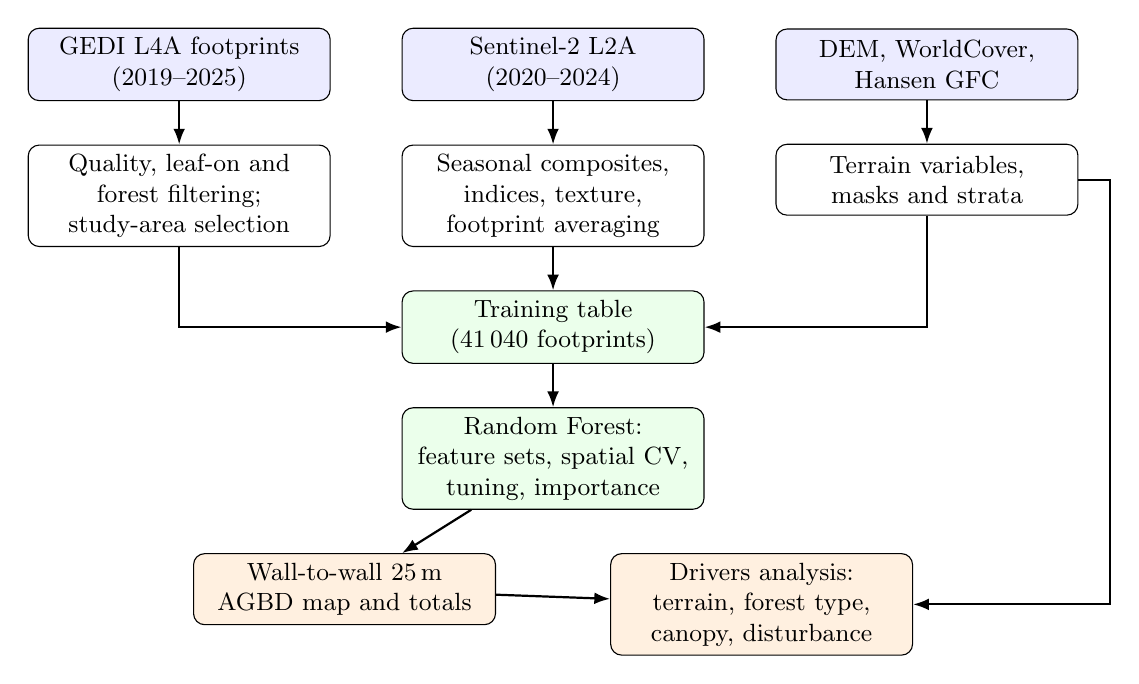
\begin{tikzpicture}[
  node distance=0.55cm and 0.9cm,
  box/.style={draw, rounded corners, align=center, font=\small, minimum height=0.9cm,
              text width=3.6cm, fill=#1},
  box/.default=white,
  arr/.style={-{Latex[length=2mm]}, thick}]
  \node[box=blue!8] (gedi) {GEDI L4A footprints\\(2019--2025)};
  \node[box=blue!8, right=of gedi] (s2) {Sentinel-2 L2A\\(2020--2024)};
  \node[box=blue!8, right=of s2] (aux) {DEM, WorldCover,\\Hansen GFC};
  \node[box, below=of gedi] (filt) {Quality, leaf-on and\\forest filtering;\\study-area selection};
  \node[box, below=of s2] (pred) {Seasonal composites,\\indices, texture,\\footprint averaging};
  \node[box, below=of aux] (terr) {Terrain variables,\\masks and strata};
  \node[box=green!8, below=of pred] (train) {Training table\\(41\,040 footprints)};
  \node[box=green!8, below=of train] (rf) {Random Forest:\\feature sets, spatial CV,\\tuning, importance};
  \node[box=orange!12, below left=0.55cm and -1.2cm of rf] (map) {Wall-to-wall 25\,m\\AGBD map and totals};
  \node[box=orange!12, below right=0.55cm and -1.2cm of rf] (drv) {Drivers analysis:\\terrain, forest type,\\canopy, disturbance};
  \draw[arr] (gedi) -- (filt);
  \draw[arr] (s2) -- (pred);
  \draw[arr] (aux) -- (terr);
  \draw[arr] (filt) |- (train);
  \draw[arr] (pred) -- (train);
  \draw[arr] (terr) |- (train);
  \draw[arr] (train) -- (rf);
  \draw[arr] (rf) -- (map);
  \draw[arr] (map) -- (drv);
  \draw[arr] (terr.east) -- ++(0.4,0) |- (drv.east);
\end{tikzpicture}
\caption{Processing workflow.}
\label{fig:workflow}
\end{figure}

\subsection{GEDI L4A filtering}

GEDI shots were kept if they satisfied the recommended L4A quality criteria
(\texttt{l4\_quality\_flag}~=~1, \texttt{degrade\_flag}~=~0,
\texttt{algorithm\_run\_flag}~=~1, sensitivity~$\geq$~0.95) and had AGBD between 0 and
500~\mgha{}. Because the forests are deciduous and GEDI's own \texttt{leaf\_off\_flag} is
always 0 over Betul, only shots acquired in the leaf-on months (July--January) were used. To
limit the effect of the $\sim$10\,m GEDI geolocation error at forest edges, a shot was kept
only if all WorldCover pixels within 20\,m of its centre were tree cover. Shots on pixels with
Hansen tree-cover loss in or after 2019 were removed, because the canopy could differ between
the GEDI acquisition and the Sentinel-2 composites. In the monthly GEDI rasters the
\texttt{lat\_lowestmode}/\texttt{lon\_lowestmode} bands are empty, so each footprint was
positioned using the geolocation of algorithm setting~1 (\texttt{*\_a1} bands), falling back
to the 25\,m pixel centre where this was missing.

\paragraph{Study-area selection.} GEDI coverage is uneven, so the district was divided into
5\,km cells (477 cells) and only cells with at least 30 filtered shots and at least 20\%
WorldCover tree cover were retained. The selected 191 cells (4\,299\,km$^2$,
Figure~\ref{fig:grid}) define the study area for modelling and mapping.

\subsection{Predictor variables}

\paragraph{Sentinel-2.} Scenes with less than 70\% cloud cover were masked with Cloud Score+
(\texttt{cs\_cdf}~$\geq$~0.6) and reduced to two seasonal median composites over 2020--2024:
a post-monsoon leaf-on composite (October--January) and a dry-season leaf-off composite
(March--May). For each season, ten bands (B2--B8A, B11, B12) and ten vegetation indices were
computed: NDVI, EVI \citep{huete2002}, SAVI \citep{huete1988}, NDMI, NBR, NDRE, the red-edge
chlorophyll index CIre \citep{gitelson2003}, MTCI \citep{dash2004}, IRECI and S2REP
\citep{frampton2013}. Seasonal differences (leaf-on minus leaf-off) of NDVI, EVI, NDMI and
NDRE describe deciduous phenology. Grey-level co-occurrence texture \citep{haralick1973}
(contrast, entropy, variance and inverse difference moment) was computed from the leaf-on NIR
band (B8, quantised to 64 levels, 5$\times$5 window). All optical predictors were averaged over
a 12.5\,m radius circle so that each training sample describes the same ground area as a
GEDI footprint.

\paragraph{Terrain.} Elevation, slope, northness ($\cos$ aspect), eastness ($\sin$ aspect)
and the topographic position index (elevation minus mean elevation within 300\,m) were
derived from the Copernicus GLO-30 DEM.

\paragraph{Feature sets.} Three nested sets were compared: (i) leaf-on Sentinel-2 bands,
indices and texture; (ii) as (i) plus the leaf-off composite and seasonal differences;
(iii) as (ii) plus terrain. Within each set, near-duplicate predictors (Pearson
$|r| > 0.98$ with an earlier predictor) were removed, e.g.\ B7, B8, B8A, SAVI and NBR of the
leaf-on composite.

\subsection{Random Forest model and validation}

AGBD was modelled with Random Forest regression \citep{breiman2001} (300 trees, bootstrap
fraction 0.632). Neighbouring GEDI footprints along a track are spatially autocorrelated, so
random $k$-fold cross-validation overestimates accuracy for prediction at new locations
\citep{roberts2017, ploton2020}. All model selection therefore used 5-fold \emph{spatial block}
cross-validation: footprints were grouped into 5\,km$\times$5\,km blocks (193 blocks) and
whole blocks were held out. Random 5-fold cross-validation is reported only for comparison.
The best feature set was chosen by spatial-CV RMSE; then the fraction of predictors tried at
each split (0.2, 0.33, 0.5) and the minimum leaf size (1, 5, 10, 20) were tuned on a
40\,000-footprint subsample. Accuracy is reported as \rsq{}, RMSE, relative RMSE (RMSE divided
by mean observed AGBD), mean absolute error and bias (mean of predicted minus observed).
Predictor importance was measured by permutation importance (decrease in \rsq{} on one
spatial hold-out fold, five repeats).

\subsection{Wall-to-wall prediction}

The selected model configuration was re-trained in Earth Engine
(\texttt{smileRandomForest}) on all footprints and applied to the predictor stack over
WorldCover tree cover in the study area at 25\,m resolution (UTM zone 43N). The full model
(300 trees, minimum leaf size 5, $\approx$1.5 million nodes) exceeds Earth Engine's limit on
model size, so the map was produced with 150 trees and a minimum leaf size of 10; in local
spatial cross-validation this reduces \rsq{} only from 0.296 to 0.293 (RMSE 47.5 to
47.6~\mgha{}). Agreement between the Earth Engine and scikit-learn implementations was checked
by training without the blocks of one spatial fold and predicting them. Total above-ground
biomass was obtained by summing AGBD$\times$pixel area and converted to carbon with a carbon
fraction of 0.47 \citep{ipcc2006}.

\subsection{Drivers of biomass variation}

The map was stratified by elevation (100\,m bands), slope (0--5, 5--10, 10--20, 20--30,
$>$30$^\circ$), aspect (N, E, S, W quadrants), canopy density (Forest Survey of India classes:
$<$10, 10--40, 40--70, $\geq$70\% tree cover, \citealp{fsi2021}) from Hansen tree cover in
2000, forest type, and disturbance history (Hansen loss year grouped as no loss, 2001--2010,
2011--2018 and 2019--2025). As no forest-type map was available, forest type was approximated
by a deciduousness index,
\begin{equation}
  D = \frac{\mathrm{NDVI}_{\text{on}} - \mathrm{NDVI}_{\text{off}}}{\mathrm{NDVI}_{\text{on}}},
\end{equation}
split into terciles (low, medium, high deciduousness) over tree cover in the study area. Zonal
statistics were computed from the full map at 50\,m. Relationships were tested with Spearman
correlation (continuous variables) and Kruskal--Wallis tests (classes) on a random sample of
17\,967 map pixels and, as an independent check, on the 41\,040 GEDI footprints themselves.

% ===========================================================================
\section{Results}

\subsection{GEDI data}

Table~\ref{tab:cascade} shows how the filters reduced the GEDI data over the district. The
quality flags removed 84\% of all shots, the leaf-on restriction another 32\% of the
remainder, and the tree-cover requirements most of what was left, leaving 44\,608 shots in the
district and 41\,040 footprints with complete predictors inside the study area. Acquisitions are
unevenly distributed in time (2020: 14\,802; 2022: 10\,739; 2023: only 712 footprints) and
within the year: few high-quality shots were acquired during the monsoon (June--August) because
of cloud, and most leaf-on footprints date from October to January.

\begin{table}[htbp]
\centering
\caption{GEDI L4A filter cascade over Betul district (2019-04 to 2025-06).}
\label{tab:cascade}
\small
\begin{tabular}{l r}
\toprule
Filter stage & Shots remaining \\
\midrule
All shots & 1\,606\,351 \\
+ quality, degrade and algorithm flags & 254\,496 \\
+ sensitivity $\geq$ 0.95 & 254\,494 \\
+ leaf-on months (July--January) & 173\,852 \\
+ AGBD range 0--500~\mgha{} & 173\,799 \\
+ in WorldCover tree cover & 62\,597 \\
+ homogeneous tree cover (20\,m radius) & 44\,616 \\
+ no Hansen loss since 2019 & 44\,608 \\
\midrule
Inside selected study area & 41\,072 \\
With complete predictors (training set) & 41\,040 \\
\bottomrule
\end{tabular}
\end{table}

\begin{figure}[htbp]
\centering
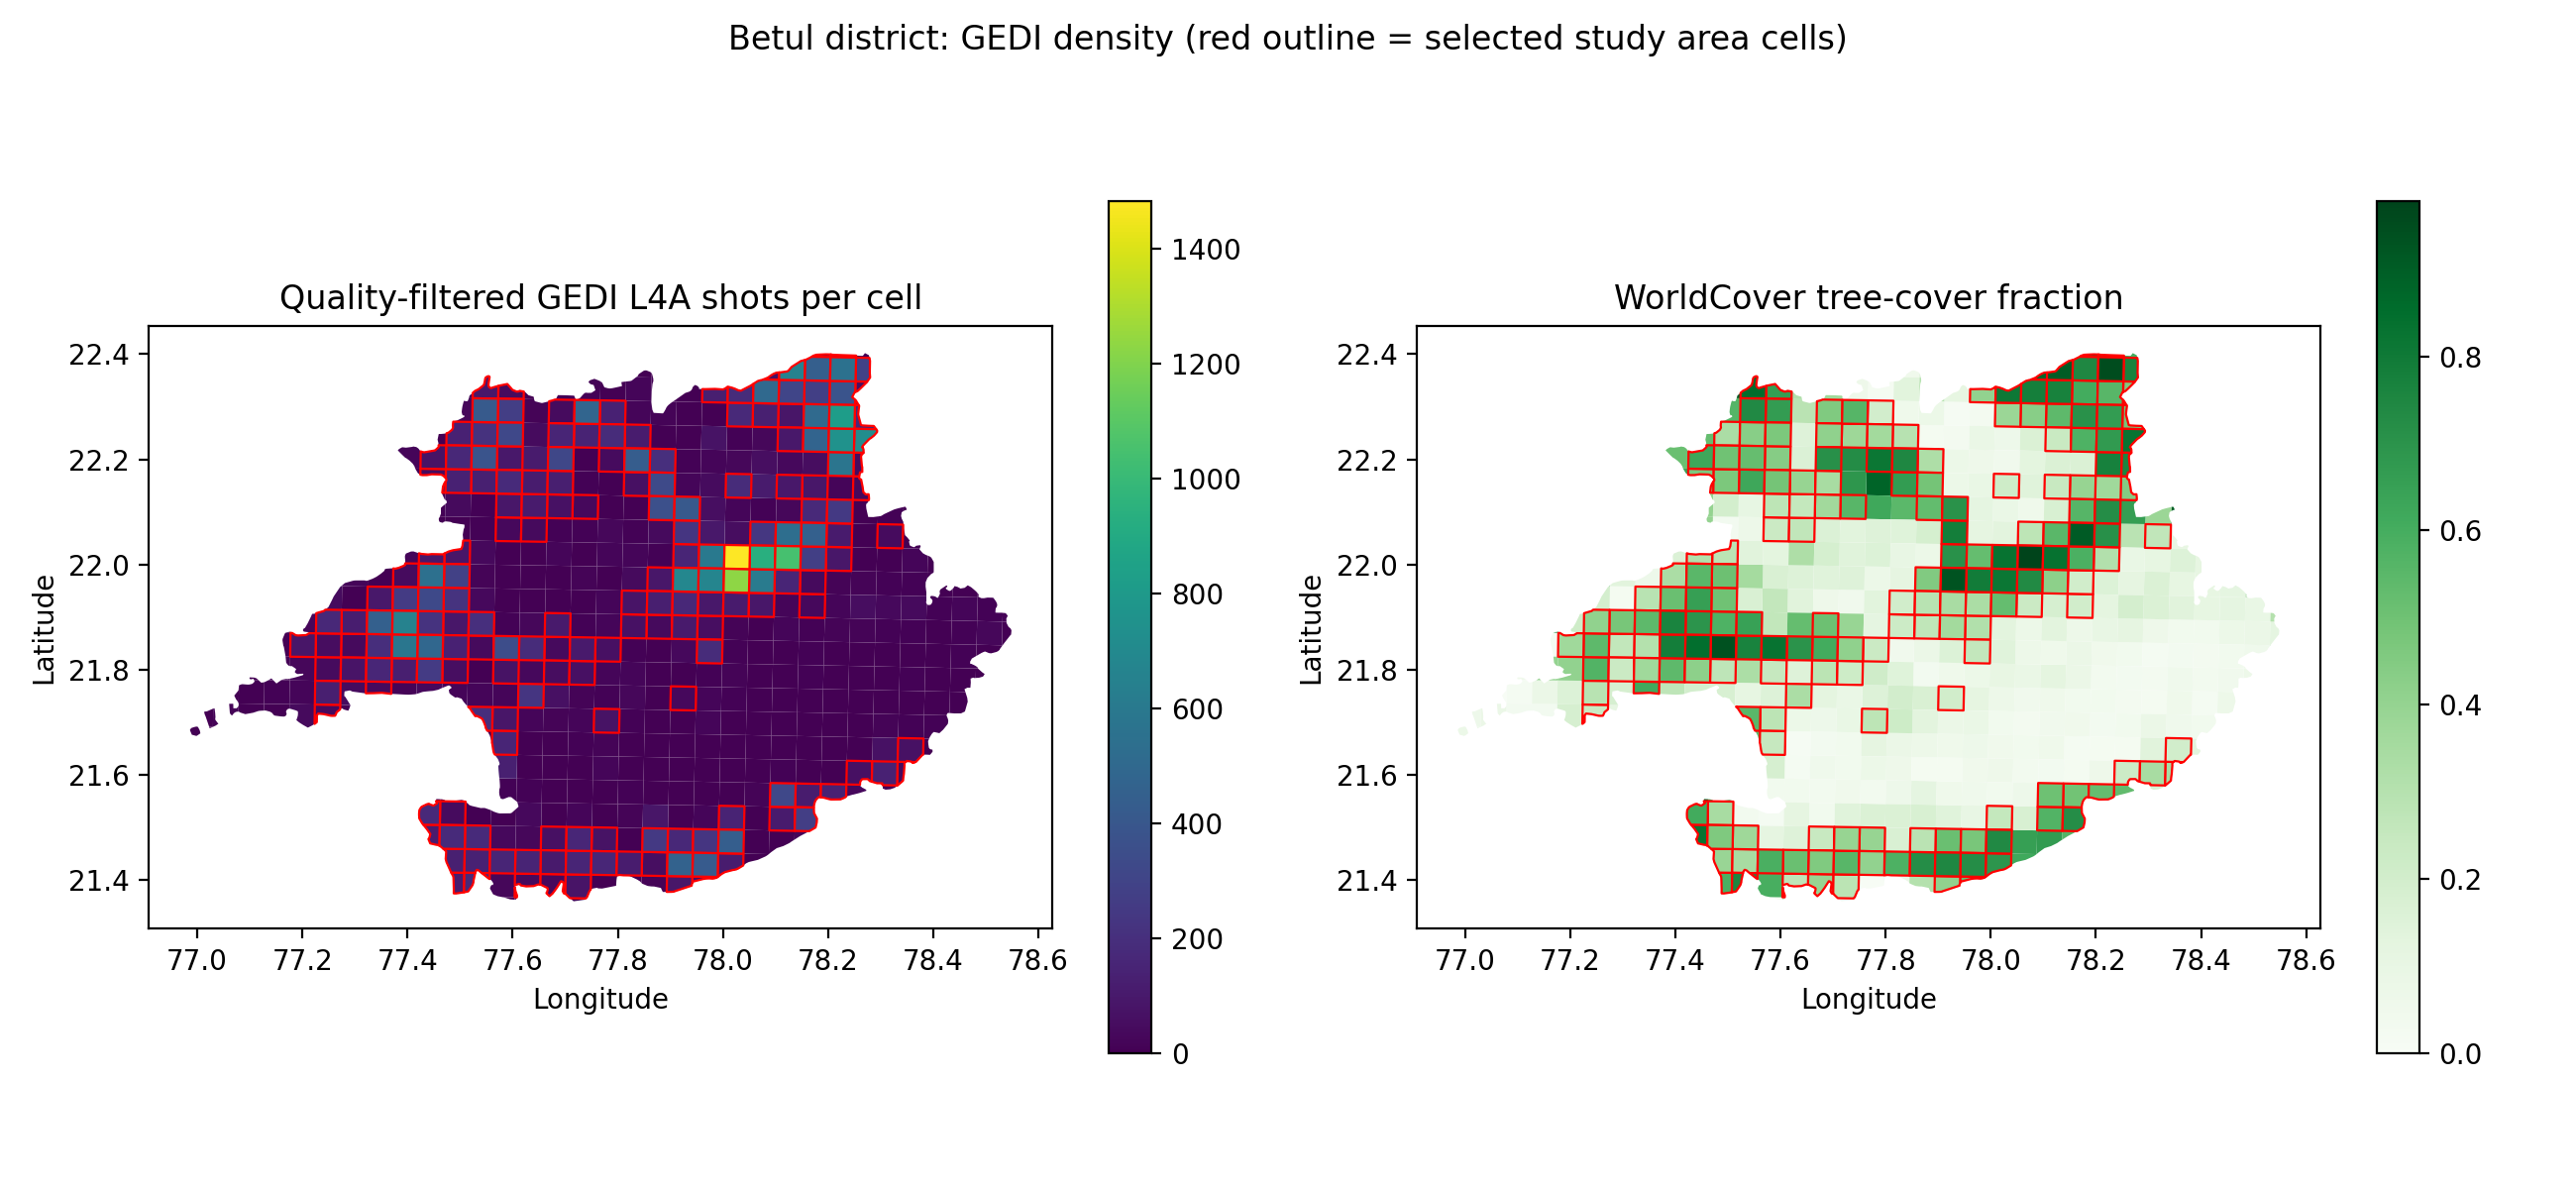
\includegraphics[width=\textwidth]{01_gedi_grid.png}
\caption{Number of filtered GEDI L4A shots (left) and WorldCover tree-cover fraction (right)
per 5\,km cell. Cells outlined in red form the study area.}
\label{fig:grid}
\end{figure}

The training footprints have a mean AGBD of 91.0~\mgha{} (median 79.5, interquartile range
47.8--122.5, maximum 487~\mgha{}; Figure~\ref{fig:gedidist}). The reported L4A standard error is
bimodal (about 3 or 17~\mgha{}), which reflects the plant functional type (PFT) assigned by
the L4A algorithm (Table~\ref{tab:pft}): only 59\% of the footprints, all of which lie in
homogeneous WorldCover tree cover, were assigned the deciduous broadleaf tree PFT; 26\% were
assigned the grass PFT and 15\% crop PFTs. Footprints assigned the grass PFT have the
\emph{highest} mean AGBD (130~\mgha{}) and the smallest standard error.

\begin{figure}[htbp]
\centering
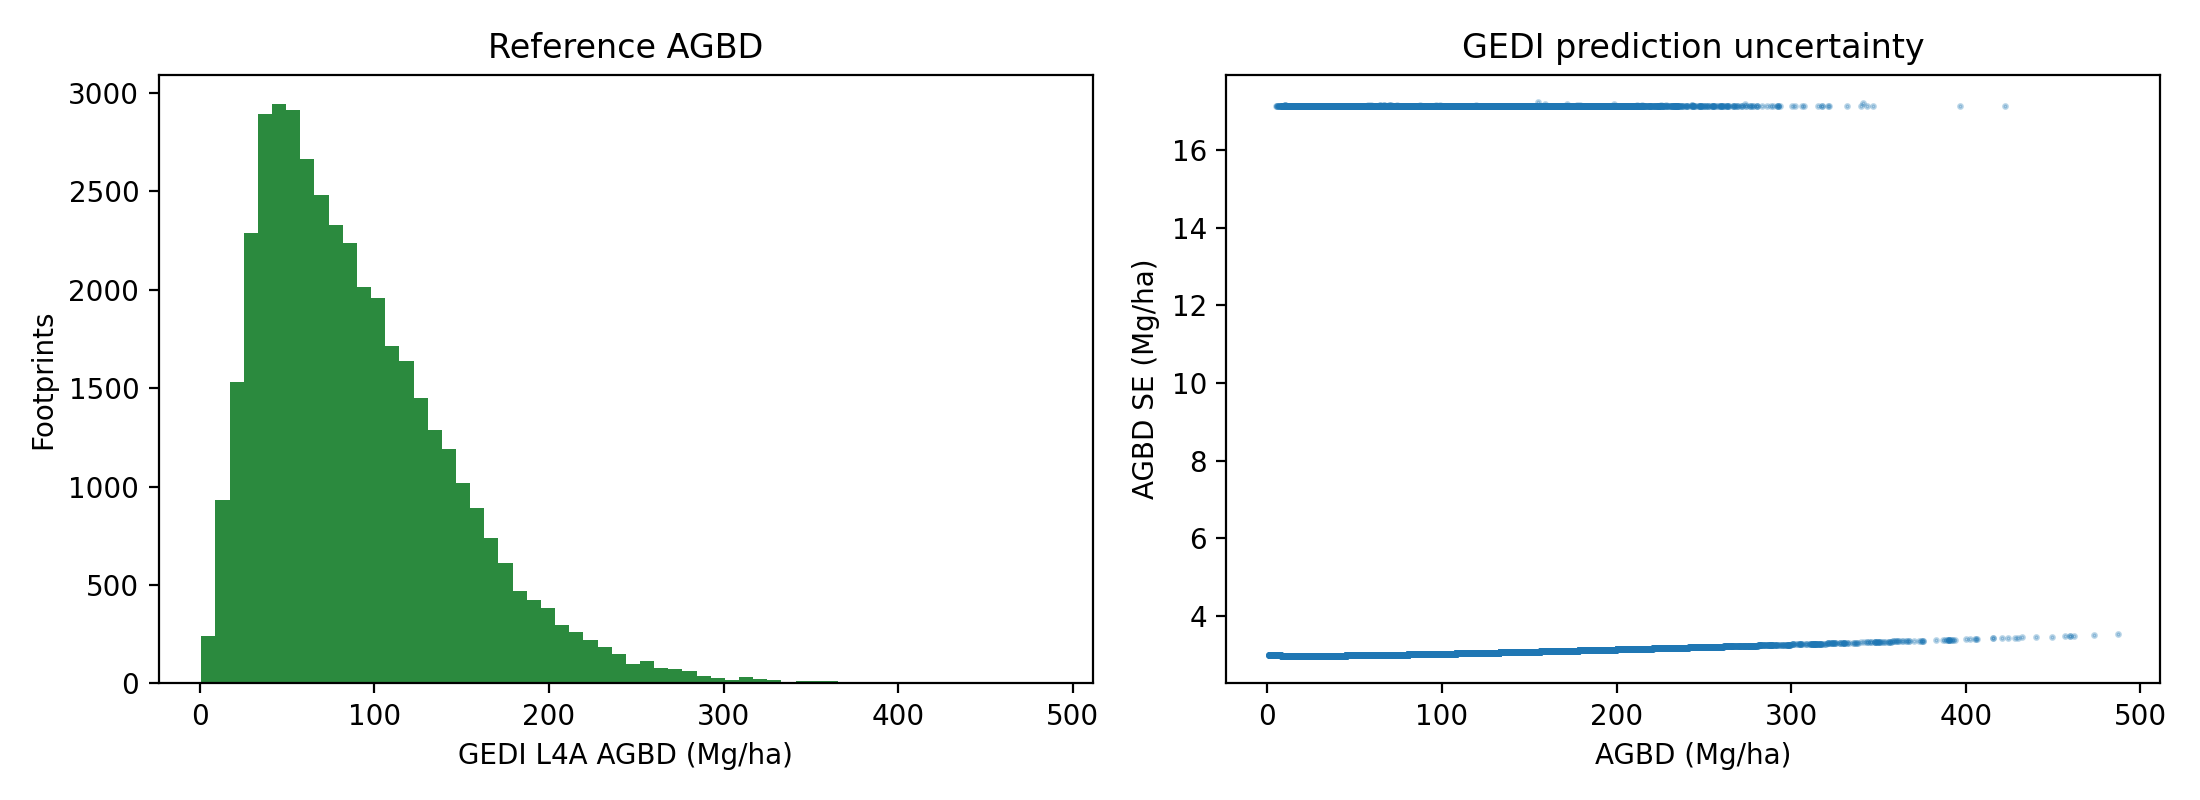
\includegraphics[width=0.95\textwidth]{03_gedi_agbd_distribution.png}
\caption{Distribution of GEDI L4A AGBD in the training set (left) and its relationship to the
L4A standard error (right).}
\label{fig:gedidist}
\end{figure}

\begin{table}[htbp]
\centering
\caption{Training footprints by GEDI L4A plant functional type (MODIS MCD12Q1 land cover
type 5 classes).}
\label{tab:pft}
\small
\begin{tabular}{l r r r r}
\toprule
PFT & Footprints & Share (\%) & Mean AGBD (\mgha{}) & Mean SE (\mgha{}) \\
\midrule
Deciduous broadleaf trees (4) & 24\,179 & 58.9 & 82.4 & 17.1 \\
Grasses (6) & 10\,859 & 26.5 & 130.2 & 3.1 \\
Cereal crops (7) & 4\,023 & 9.8 & 58.4 & 9.5 \\
Broadleaf crops (8) & 1\,954 & 4.8 & 46.1 & 14.3 \\
Other (2, 9) & 25 & 0.1 & -- & -- \\
\bottomrule
\end{tabular}
\end{table}

\subsection{Model performance}

Table~\ref{tab:featsets} compares the feature sets. Adding the leaf-off composite and the
seasonal differences reduced RMSE by 1.2~\mgha{} (\rsq{} 0.21~$\rightarrow$~0.24), and adding
terrain reduced it by a further 1.8~\mgha{} (\rsq{}~=~0.30). The two-season plus terrain set
(43 predictors) was selected. Hyper-parameters had little influence: RMSE varied only between
47.5 and 48.0~\mgha{} over the tuning grid, and the best configuration (50\% of predictors per
split, minimum leaf size 5) was used.

\begin{table}[htbp]
\centering
\caption{Spatial block cross-validation (5 folds, 5\,km blocks, $n=41\,040$) for the three
feature sets, and random cross-validation for the selected set.}
\label{tab:featsets}
\small
\begin{tabular}{l c c c c c c}
\toprule
Feature set & Predictors & \rsq{} & RMSE & rRMSE (\%) & MAE & Bias \\
\midrule
S2 leaf-on & 18 & 0.205 & 50.4 & 55.5 & 38.5 & 0.8 \\
S2 two-season & 38 & 0.242 & 49.3 & 54.2 & 37.5 & 1.1 \\
\textbf{S2 two-season + terrain} & \textbf{43} & \textbf{0.296} & \textbf{47.5} &
  \textbf{52.2} & \textbf{35.9} & \textbf{1.2} \\
\midrule
\multicolumn{7}{l}{\textit{Selected set, random 5-fold CV (optimistic)}} \\
S2 two-season + terrain & 43 & 0.342 & 45.9 & 50.4 & 34.3 & 0.6 \\
\bottomrule
\multicolumn{7}{l}{\footnotesize RMSE, MAE and bias in \mgha{}; bias = mean(predicted $-$
observed). The selected set uses tuned hyper-parameters.}
\end{tabular}
\end{table}

Figure~\ref{fig:cv} shows the cross-validated predictions. The model is nearly unbiased overall
(1.2~\mgha{}) but compresses the range of AGBD: low-biomass footprints are overestimated and
high-biomass footprints underestimated (Table~\ref{tab:range}). Errors are smallest between 75
and 100~\mgha{} (RMSE 24.9~\mgha{}), close to the mean of the data, and grow rapidly above
150~\mgha{}, where predictions saturate at around 150--190~\mgha{}.

\begin{figure}[htbp]
\centering
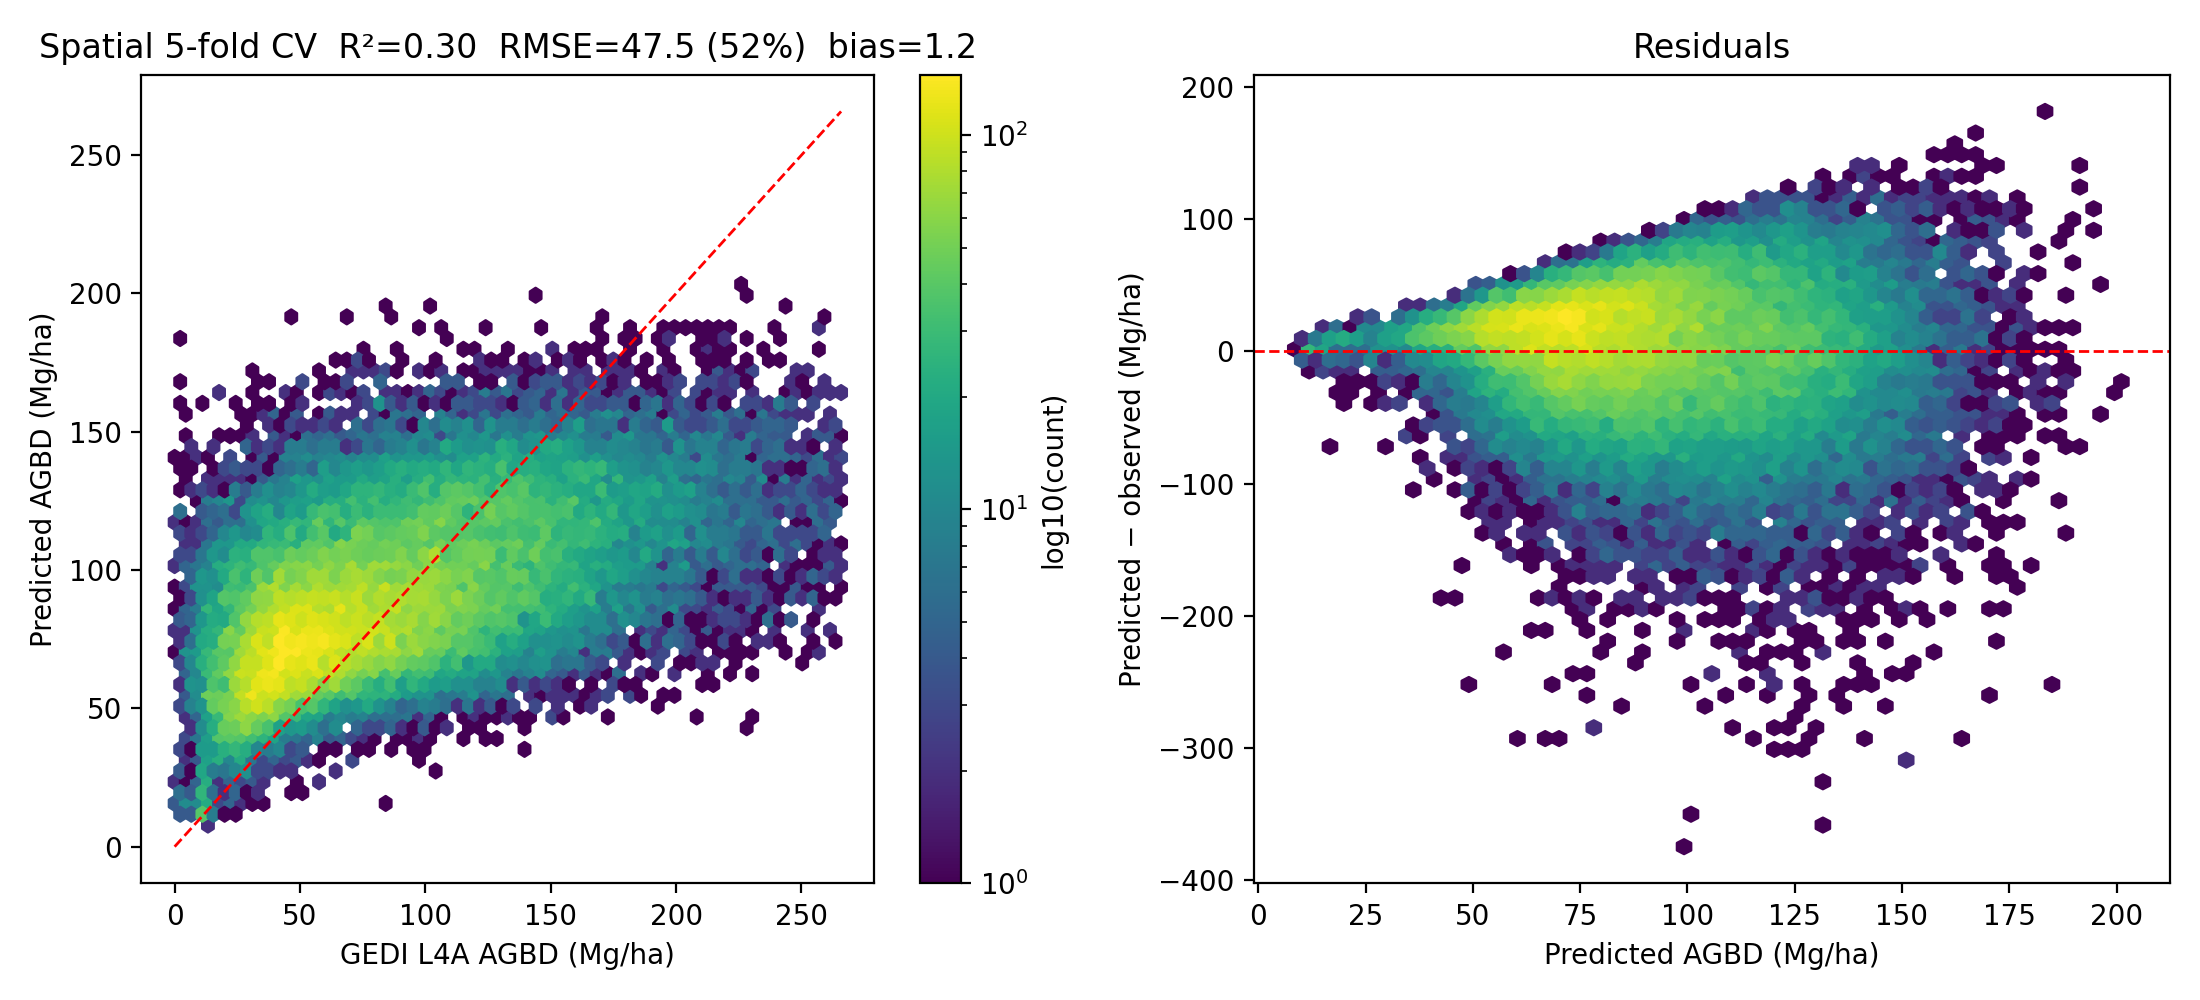
\includegraphics[width=\textwidth]{03_cv_scatter_S2_twoseason_terrain.png}
\caption{Spatial cross-validation of the selected model: predicted versus GEDI L4A AGBD (left;
dashed line 1:1) and residuals versus prediction (right).}
\label{fig:cv}
\end{figure}

\begin{table}[htbp]
\centering
\caption{Spatial cross-validation error by GEDI AGBD range.}
\label{tab:range}
\small
\begin{tabular}{l r r r}
\toprule
AGBD range (\mgha{}) & Footprints & RMSE (\mgha{}) & Bias (\mgha{}) \\
\midrule
0--25 & 2\,667 & 56.6 & +49.1 \\
25--50 & 8\,359 & 42.7 & +36.6 \\
50--75 & 8\,235 & 32.6 & +23.3 \\
75--100 & 6\,666 & 24.9 & +6.0 \\
100--150 & 9\,207 & 32.4 & $-$18.8 \\
150--200 & 3\,948 & 61.4 & $-$55.3 \\
200--300 & 1\,772 & 112.2 & $-$106.9 \\
$>$300 & 186 & 219.9 & $-$214.8 \\
\bottomrule
\end{tabular}
\end{table}

Slope was by far the most important predictor (Figure~\ref{fig:imp}): permuting it reduced
\rsq{} by 0.14, three times more than any other variable. It was followed by the leaf-on
red-edge position (S2REP), NIR texture contrast, elevation, dry-season blue reflectance and
leaf-on red and red-edge reflectance. Red-edge variables and texture were generally more
important than broadband greenness indices such as NDVI and EVI.

\begin{figure}[htbp]
\centering
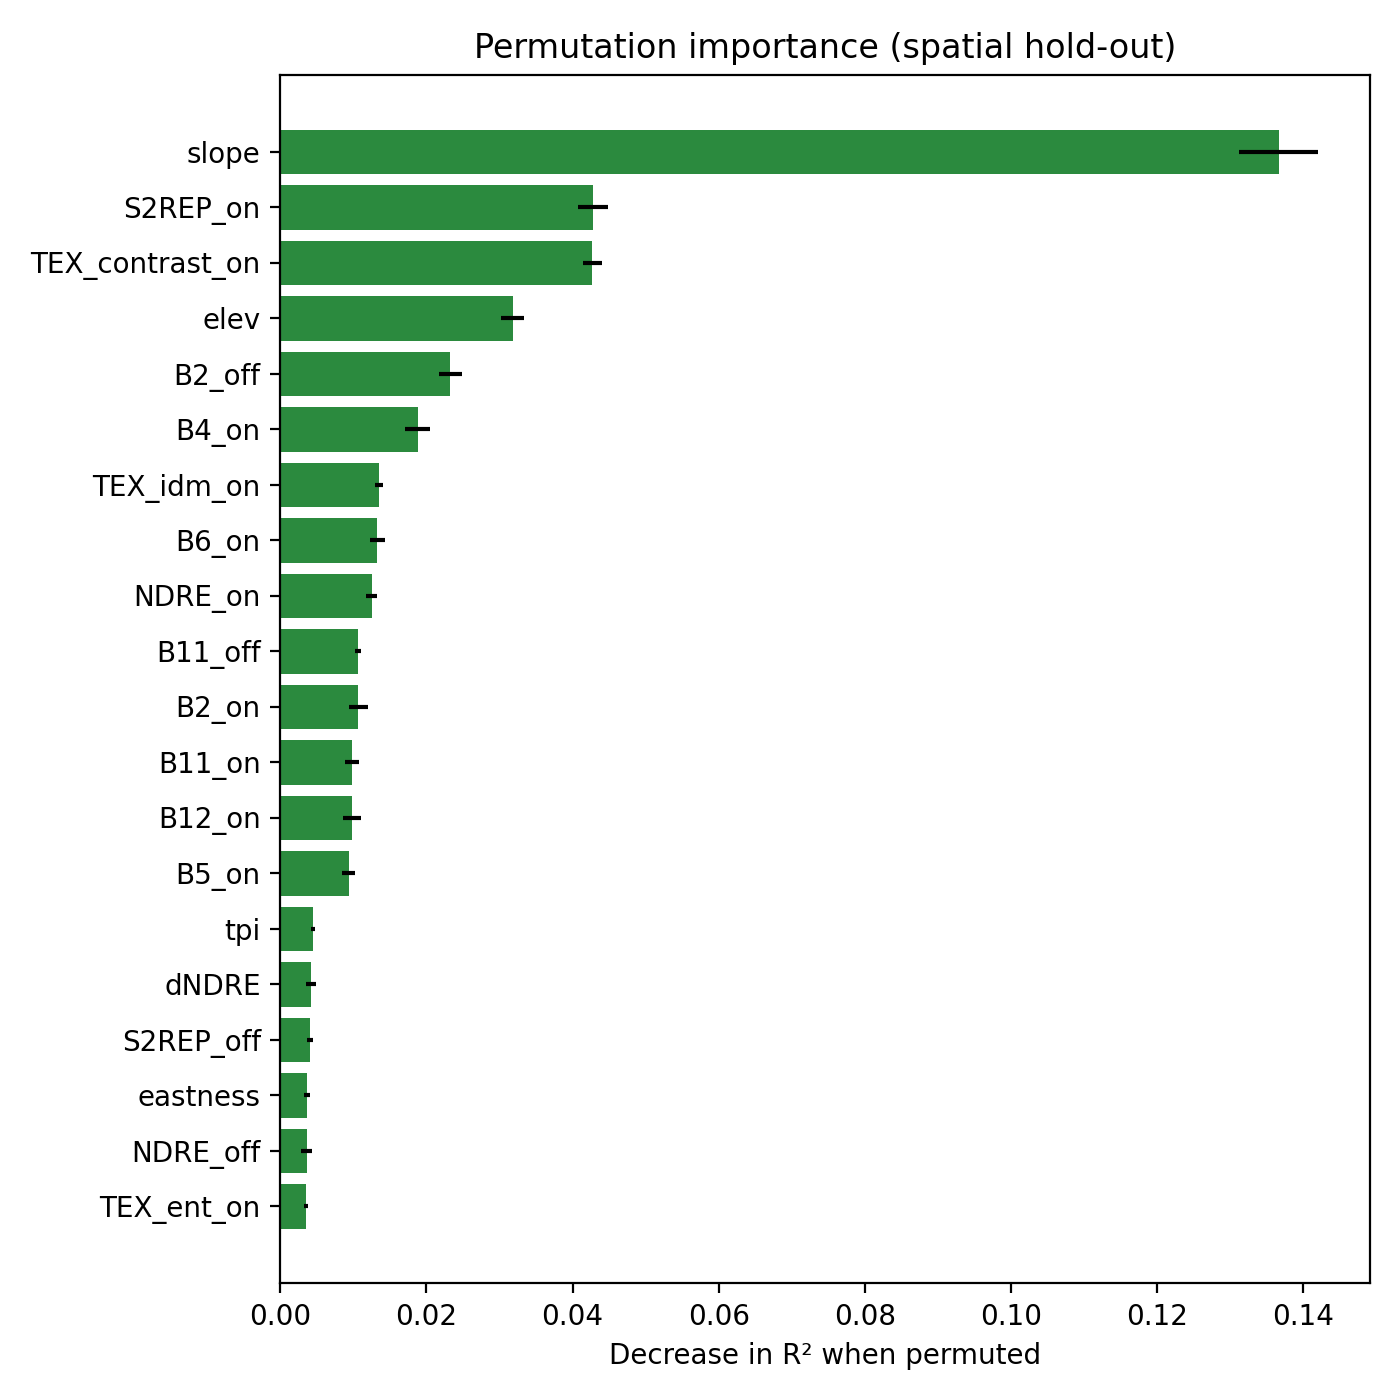
\includegraphics[width=0.62\textwidth]{03_permutation_importance.png}
\caption{Permutation importance (decrease in \rsq{}) of the 20 most important predictors on
a spatial hold-out fold. Suffixes \texttt{\_on}/\texttt{\_off}: leaf-on/leaf-off composite;
\texttt{TEX}: GLCM texture of leaf-on NIR.}
\label{fig:imp}
\end{figure}

\paragraph{Earth Engine implementation.} Trained without the 38 blocks of the first spatial
fold, the reduced Earth Engine forest predicted those 8\,224 footprints with \rsq{}~=~0.32 and
RMSE~=~48.2~\mgha{}, consistent with the local spatial cross-validation.

\subsection{Biomass map}

Figure~\ref{fig:map} shows the predicted AGBD. Higher values (often $>$120~\mgha{}) occur in
the hilly forests in the west and north-west of the district and along the ridges in the
centre-east, while the forests of the central plateau and the north-east have lower values.
Over the 213\,795\,ha of WorldCover tree cover in the study area the mean predicted AGBD is
89.9~\mgha{}, giving a total above-ground biomass of 19.2~Tg and a carbon stock of
approximately 9.0~Tg~C (Table~\ref{tab:totals}). The mean is close to the mean of the GEDI
training data (91.0~\mgha{}), but the map has a much narrower distribution, as expected from
the cross-validation results.

\begin{figure}[htbp]
\centering
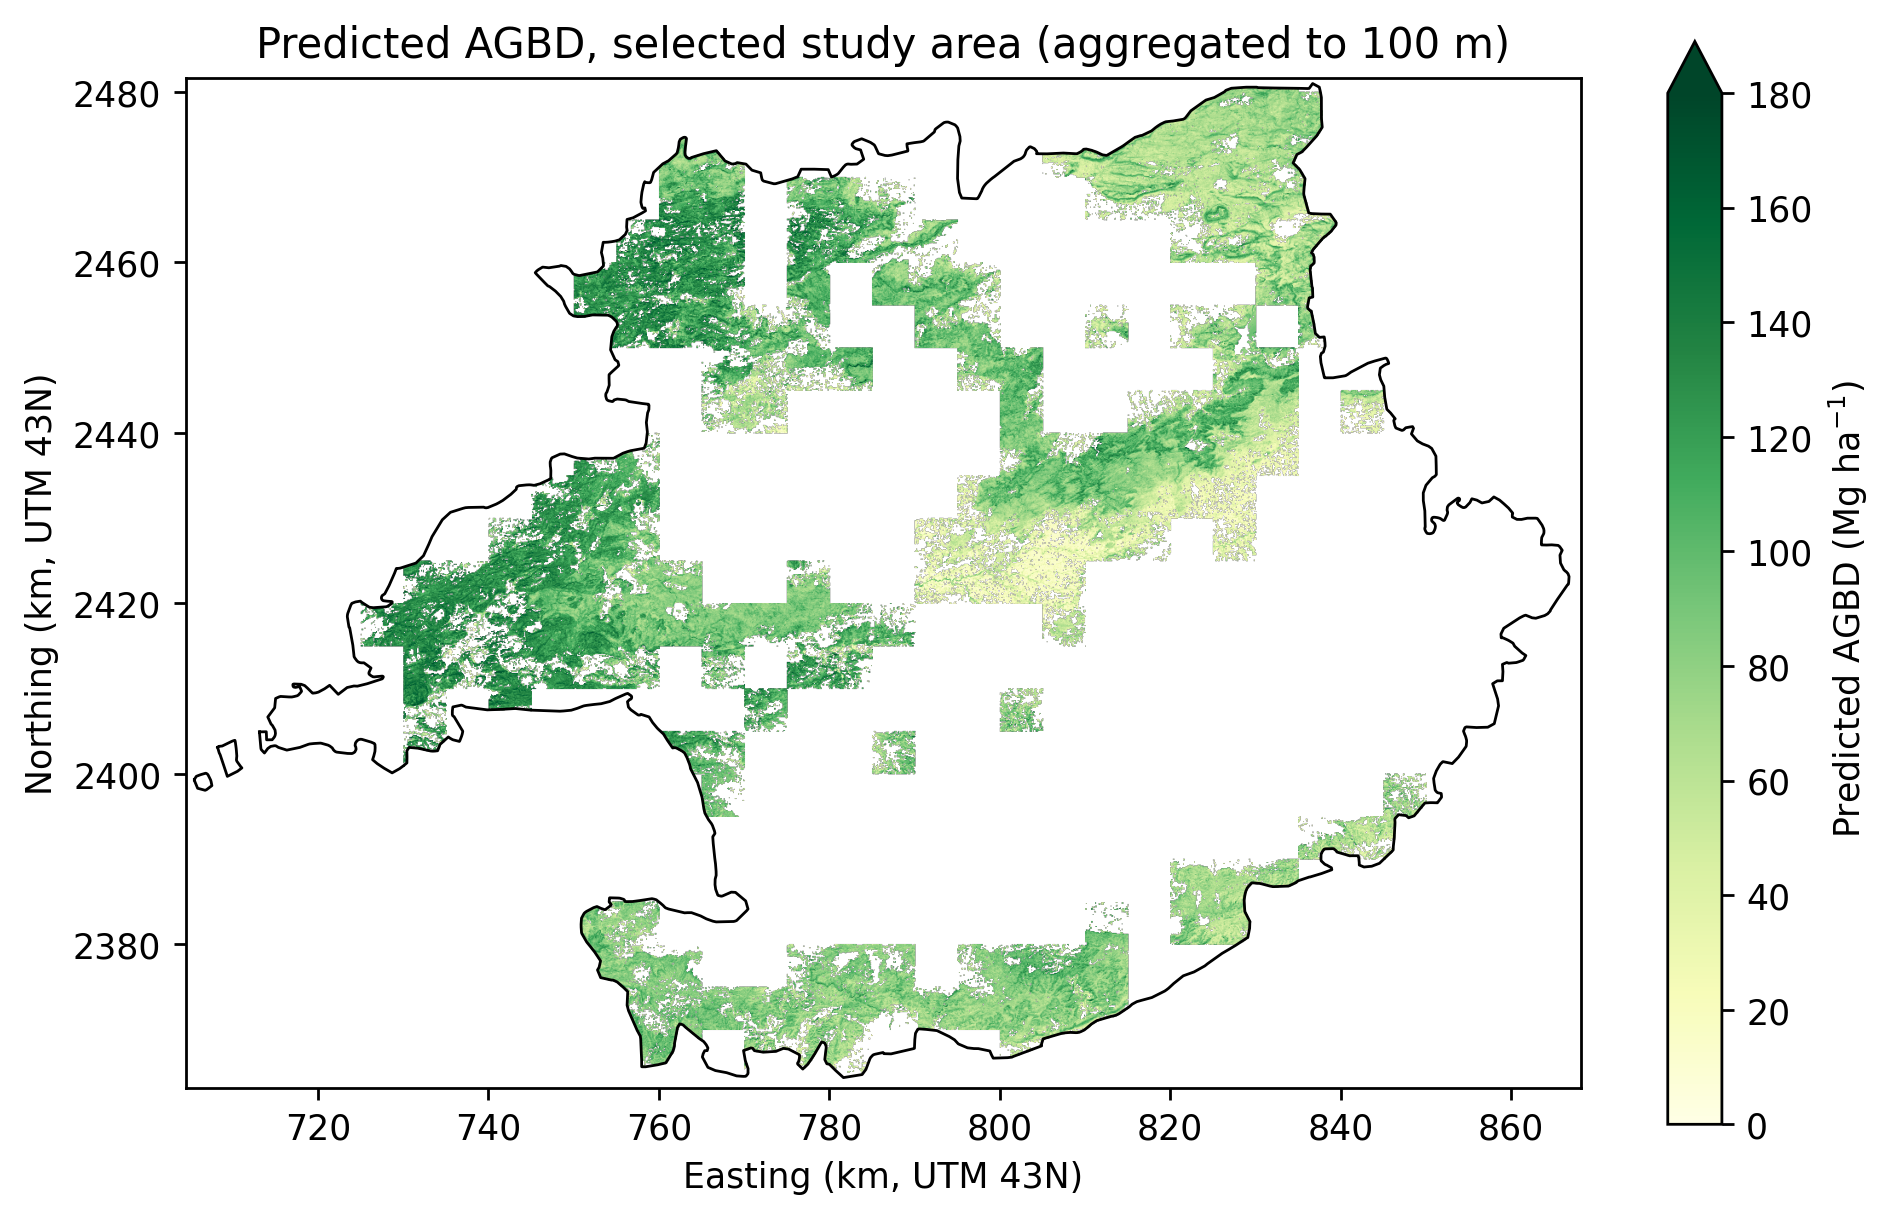
\includegraphics[width=0.9\textwidth]{04_agbd_map.png}
\caption{Predicted AGBD over tree cover in the study area (25\,m map aggregated to 100\,m for
display). Black line: Betul district boundary; white areas inside the boundary are non-forest
or lie outside the selected cells.}
\label{fig:map}
\end{figure}

\begin{table}[htbp]
\centering
\caption{Biomass totals for tree cover in the study area.}
\label{tab:totals}
\small
\begin{tabular}{l r}
\toprule
Tree-cover area mapped & 213\,795 ha \\
Mean AGBD & 89.9 \mgha{} \\
Total above-ground biomass & 19.2 Tg \\
Above-ground carbon (CF = 0.47) & 9.0 Tg C \\
\bottomrule
\end{tabular}
\end{table}

\subsection{Drivers of biomass variation}

Table~\ref{tab:zonal} summarises predicted AGBD by stratum, Table~\ref{tab:tests} gives the
statistical tests, and Figures~\ref{fig:terrain} and~\ref{fig:strata} compare the map with the
GEDI observations.

\begin{table}[htbp]
\centering
\caption{Predicted AGBD by stratum (full-map zonal statistics at 50\,m). Share = share of
mapped tree-cover pixels.}
\label{tab:zonal}
\small
\begin{tabular}{l l r r r}
\toprule
Factor & Class & Share (\%) & Mean (\mgha{}) & SD (\mgha{}) \\
\midrule
\multirow{9}{*}{Elevation (m)}
 & 300--400 & 1.7 & 103.9 & 38.4 \\
 & 400--500 & 28.4 & 96.3 & 31.7 \\
 & 500--600 & 32.6 & 98.8 & 26.4 \\
 & 600--700 & 22.0 & 80.2 & 30.6 \\
 & 700--800 & 10.2 & 68.1 & 24.6 \\
 & 800--900 & 2.9 & 71.8 & 20.0 \\
 & 900--1000 & 1.4 & 82.1 & 19.5 \\
 & 1000--1100 & 0.7 & 72.7 & 19.9 \\
 & $>$1100 & 0.1 & 65.5 & 12.3 \\
\midrule
\multirow{5}{*}{Slope}
 & 0--5$^\circ$ & 28.3 & 74.9 & 32.0 \\
 & 5--10$^\circ$ & 25.8 & 88.4 & 27.6 \\
 & 10--20$^\circ$ & 29.9 & 95.7 & 28.0 \\
 & 20--30$^\circ$ & 13.8 & 103.8 & 25.7 \\
 & $>$30$^\circ$ & 2.1 & 115.0 & 19.4 \\
\midrule
\multirow{4}{*}{Aspect}
 & North & 29.4 & 93.0 & 33.0 \\
 & East & 19.5 & 88.1 & 30.3 \\
 & South & 28.1 & 89.4 & 29.7 \\
 & West & 23.0 & 88.0 & 30.2 \\
\midrule
\multirow{3}{*}{Forest type (proxy)}
 & Low deciduousness & 41.9 & 79.6 & 30.1 \\
 & Medium deciduousness & 28.2 & 91.8 & 27.5 \\
 & High deciduousness & 29.8 & 102.8 & 28.8 \\
\midrule
\multirow{4}{*}{\shortstack[l]{Canopy density\\(Hansen 2000)}}
 & $<$10\% & 55.5 & 87.5 & 33.0 \\
 & Open (10--40\%) & 37.4 & 94.0 & 28.3 \\
 & Moderately dense (40--70\%) & 7.0 & 83.8 & 22.7 \\
 & Very dense ($\geq$70\%) & 0.1 & 85.0 & 21.4 \\
\midrule
\multirow{4}{*}{Disturbance}
 & No loss & 99.6 & 90.0 & 31.0 \\
 & Loss 2001--2010 & 0.3 & 62.4 & 17.1 \\
 & Loss 2011--2018 & 0.1 & 89.9 & 23.3 \\
 & Loss 2019--2025 & 0.1 & 57.9 & 21.7 \\
\bottomrule
\end{tabular}
\end{table}

\begin{table}[htbp]
\centering
\caption{Spearman correlations ($\rho$) and Kruskal--Wallis statistics ($H$) between AGBD and
explanatory variables, for the map pixel sample ($n=17\,967$) and the GEDI footprints
($n=41\,040$). Unless marked, $p<0.001$.}
\label{tab:tests}
\small
\begin{tabular}{l l r r}
\toprule
Variable & Test & Map & GEDI observed \\
\midrule
Elevation & $\rho$ & $-0.29$ & $-0.15$ \\
Slope & $\rho$ & $0.38$ & $0.22$ \\
TPI & $\rho$ & $-0.09$ & $-0.05$ \\
Northness & $\rho$ & $0.03$ & $0.01$ (n.s., $p=0.28$) \\
Tree cover 2000 (Hansen) & $\rho$ & $0.12$ & $0.02$ \\
Deciduousness & $\rho$ & $0.39$ & $0.14$ \\
Canopy density class & $H$ & 301 & 269 \\
Disturbance period & $H$ & 47 & 62 \\
Slope class & $H$ & 2378 & -- \\
Forest type (proxy) & $H$ & 2144 & -- \\
\bottomrule
\end{tabular}
\end{table}

\begin{figure}[htbp]
\centering
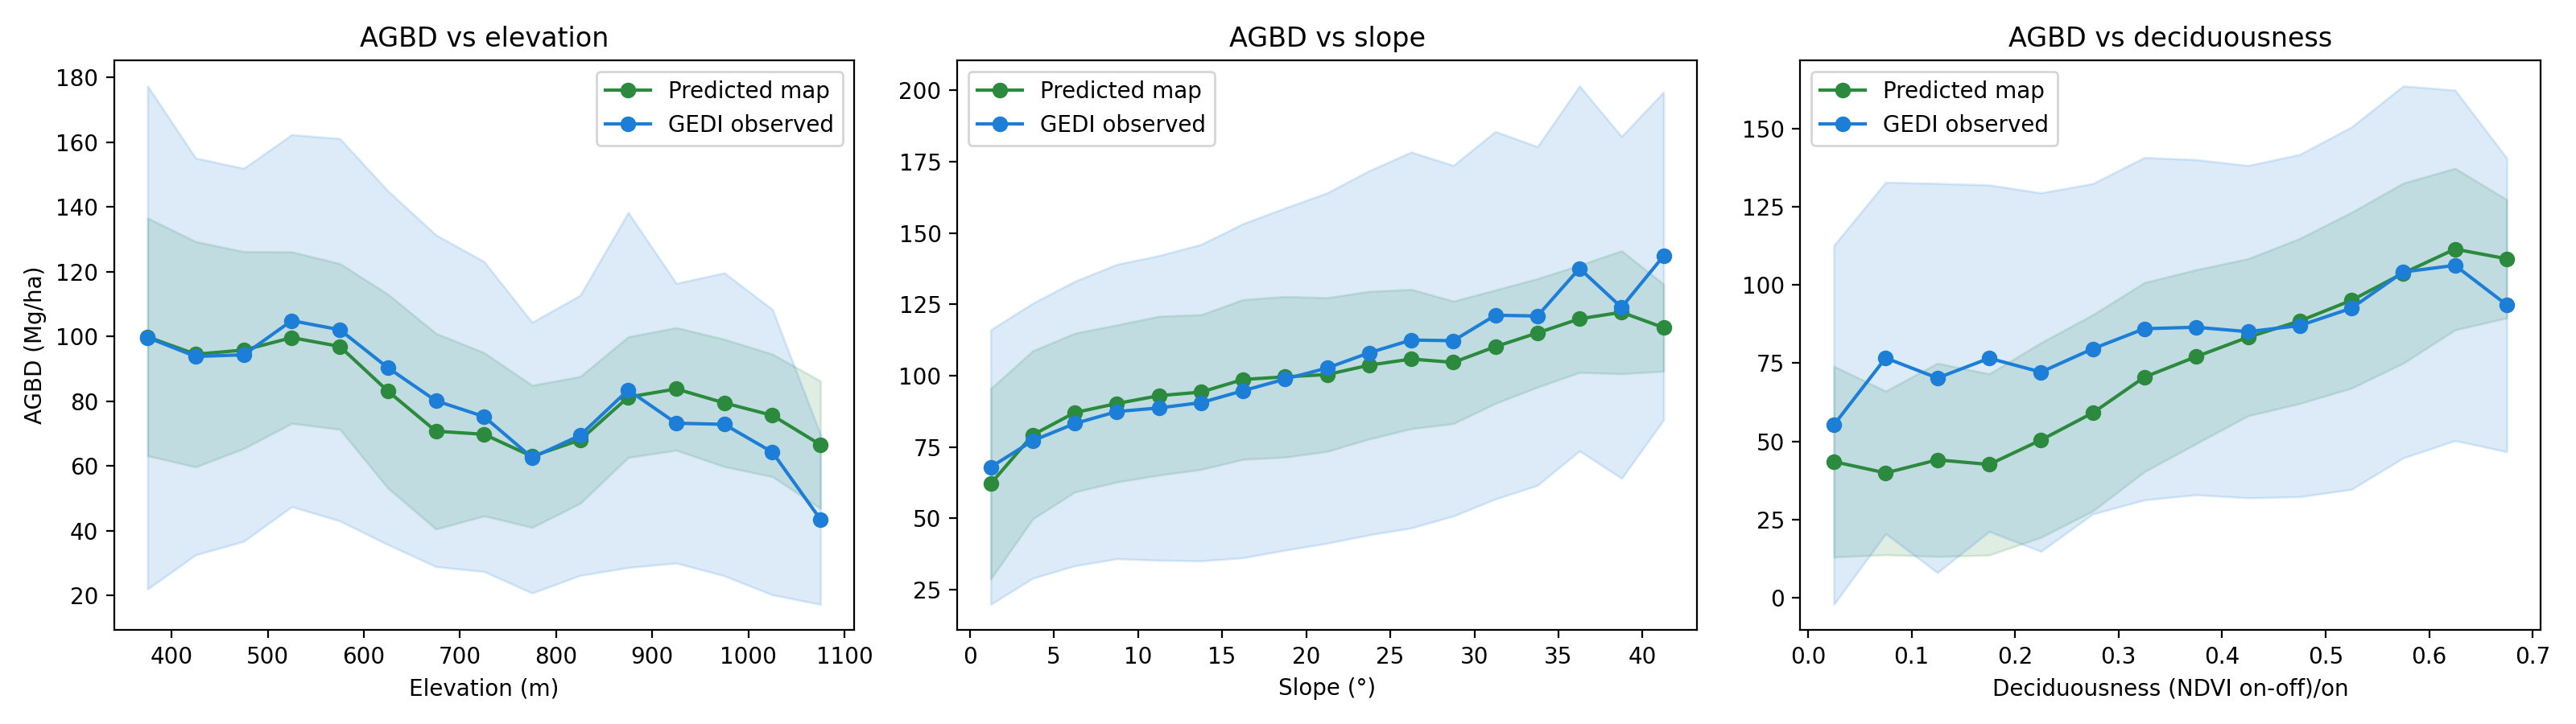
\includegraphics[width=\textwidth]{05_terrain_phenology.png}
\caption{Mean AGBD ($\pm$1 SD) as a function of elevation, slope and deciduousness for the
predicted map (green) and the GEDI footprints (blue).}
\label{fig:terrain}
\end{figure}

\begin{figure}[htbp]
\centering
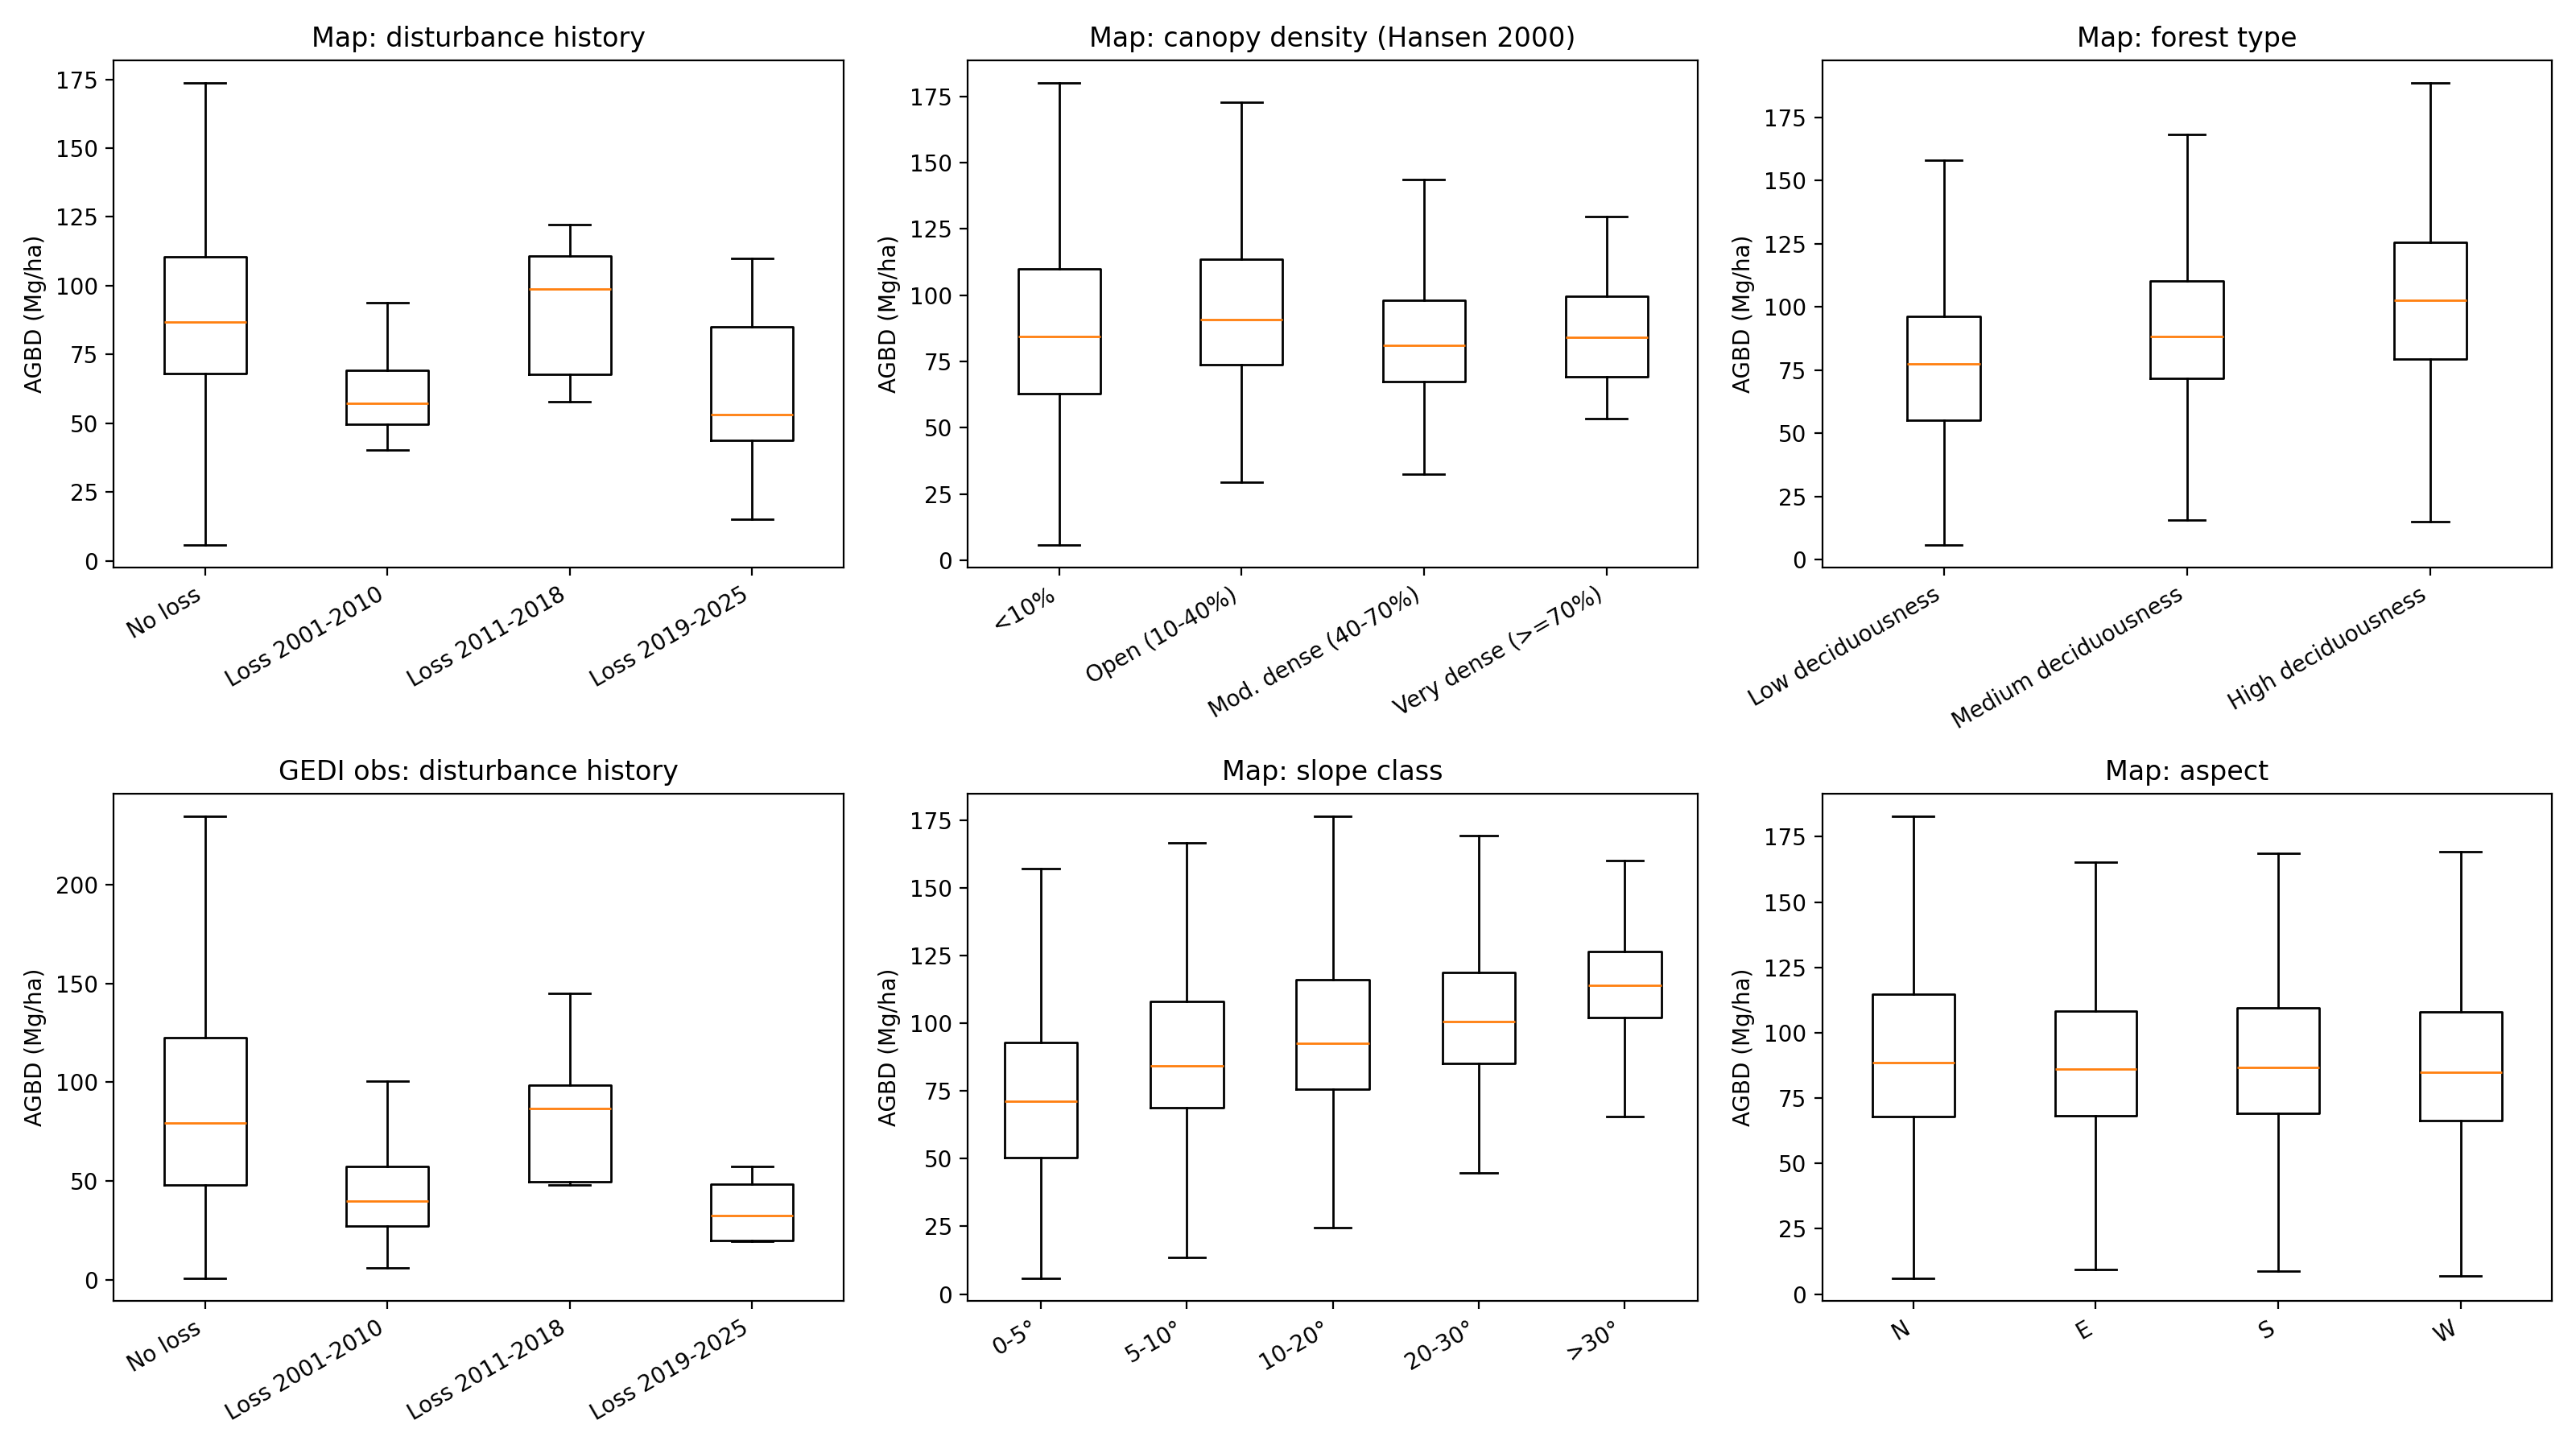
\includegraphics[width=\textwidth]{05_strata_boxplots.png}
\caption{Distribution of AGBD by disturbance history (map and GEDI observations), canopy
density, forest-type proxy, slope class and aspect (boxes: interquartile range; whiskers:
1.5$\times$IQR; outliers not shown).}
\label{fig:strata}
\end{figure}

\paragraph{Terrain.} Slope is the strongest terrain control: mean predicted AGBD rises
monotonically from 74.9~\mgha{} on slopes below 5$^\circ$ to 115.0~\mgha{} above 30$^\circ$, and
the GEDI observations show the same trend (Figure~\ref{fig:terrain}). Biomass decreases with
elevation, mainly between 500--600\,m ($\approx$99~\mgha{}) and 700--800\,m (68~\mgha{}), with a
secondary increase at 900--1000\,m. Aspect has almost no effect (88--93~\mgha{}), and the
relationship with northness is negligible in both datasets.

\paragraph{Forest type.} AGBD increases with the deciduousness index, from 79.6~\mgha{} in the
least deciduous to 102.8~\mgha{} in the most deciduous tercile. The GEDI footprints show the same
direction but a weaker relationship ($\rho=0.14$ versus 0.39), and the map underestimates GEDI
AGBD for the least deciduous pixels (Figure~\ref{fig:terrain}, right).

\paragraph{Canopy density.} Hansen tree cover in 2000 is only weakly related to AGBD
($\rho=0.12$ for the map, 0.02 for GEDI), and AGBD does not increase across the FSI density
classes. More than half of the WorldCover tree-cover pixels have less than 10\% Hansen tree
cover, so this layer appears to describe the dry deciduous canopy poorly (see
Section~\ref{sec:disc}).

\paragraph{Disturbance.} Less than 0.5\% of the mapped tree cover has a Hansen loss record.
Areas cleared in 2001--2010 have a mean AGBD of 62.4~\mgha{} and areas cleared in 2019--2025
57.9~\mgha{}, compared with 90.0~\mgha{} in undisturbed forest. Areas cleared in 2011--2018 have
biomass similar to undisturbed forest (89.9~\mgha{}), but this class covers only about 0.1\% of the
area. The GEDI footprints show the same contrast between undisturbed forest and forest cleared in
2001--2010 (Figure~\ref{fig:strata}).

% ===========================================================================
\section{Discussion}
\label{sec:disc}

\paragraph{Model accuracy.} A spatially cross-validated \rsq{} of 0.30 (RMSE 52\%) shows that
Sentinel-2 and terrain variables explain only part of the footprint-level variation in GEDI
AGBD. Several factors contribute. First, the reference data are themselves noisy: L4A AGBD is a
model prediction from a single waveform, subject to geolocation error and waveform noise, so
part of the residual variance is not predictable from any image. Second, there is a temporal
mismatch between individual GEDI acquisitions (2019--2025) and the multi-year Sentinel-2 medians
(2020--2024). Third, optical reflectance responds mainly to the upper canopy and saturates at
moderate biomass, which explains the strong underestimation above 150~\mgha{}
(Table~\ref{tab:range}). The small difference between random and spatial cross-validation
(\rsq{} 0.34 versus 0.30) indicates that spatial autocorrelation inflates random-CV accuracy
only moderately here, but spatial CV remains the appropriate estimate for a wall-to-wall map.

\paragraph{Value of phenology and terrain.} The dry-season composite improved accuracy over a
leaf-on-only model, confirming that deciduous phenology carries information about stand
structure in these forests. Red-edge variables (S2REP, NDRE, B5, B6) and NIR texture were more
important than NDVI or EVI, consistent with their lower sensitivity to saturation. Terrain
improved accuracy the most of all additions, and slope was the single most important
predictor. This should be interpreted with care. Steep slopes in Betul are less accessible and
probably less affected by cutting, grazing and conversion, which would produce a genuine
association between slope and biomass. However, terrain slope also broadens GEDI waveforms and
can bias waveform-derived height and biomass metrics upward, so part of the slope effect may be
inherited from the reference data rather than reflect real biomass differences.

\paragraph{Totals and representativeness.} The map's mean AGBD (89.9~\mgha{}) is close to that of
the training data, so aggregate totals are less affected by the range compression than
individual pixels: overestimates in low-biomass forest partly cancel underestimates in
high-biomass forest. However, training footprints were restricted to homogeneous, undisturbed
forest interiors, whereas the map covers all WorldCover tree pixels, including edges and
fragmented woodland. Predictions there are extrapolations and are probably less reliable.
% TODO: compare the 89.9 Mg/ha mean / 19.2 Tg total with published estimates for Betul or
% Central Indian dry deciduous forests (e.g. FSI ISFR carbon stock, GEDI L4B 1 km gridded AGBD).

\paragraph{GEDI plant functional types.} The L4A algorithm selects its biomass model by plant
functional type, taken from a coarse-resolution MODIS land-cover product. Although every
training footprint lies in homogeneous tree cover at 10\,m resolution, 41\% were assigned grass
or crop PFTs, presumably because the 500\,m MODIS pixels are mixed. These footprints were
therefore processed with different allometric models, and the grass-PFT footprints have
markedly higher AGBD and lower reported uncertainty than the deciduous-broadleaf footprints
(Table~\ref{tab:pft}). This inconsistency in the reference data is likely to add noise, and
possibly bias, to the model and the map.

\paragraph{Drivers.} The decrease of biomass at 600--800\,m probably corresponds to the forests
of the central plateau, which in the map appear more fragmented and interspersed with
non-forest land, while the hill forests of the west and north-west carry the highest biomass;
greater human pressure on the plateau is a plausible but untested explanation. The positive relationship with
deciduousness is opposite to the expectation that moister, less deciduous forests store more
biomass. A plausible explanation is that low deciduousness in this landscape often indicates
open or degraded woodland whose dry-season greenness comes from understorey, weeds or adjacent
irrigated land rather than from an evergreen tree canopy; this proxy should not be equated
with Champion and Seth forest types. The map relationship is also partly circular, because the
seasonal NDVI difference is itself a model predictor; the weaker relationship in the GEDI
observations is the more trustworthy estimate. Hansen tree cover for 2000 classifies more than
half of the forest as having less than 10\% canopy cover, which is inconsistent with WorldCover
and suggests that it underestimates canopy cover in leaf-off-prone dry deciduous forest; the
canopy-density results should therefore not be over-interpreted. The lower biomass of forest
cleared in 2001--2010 and the similarity of 2011--2018 clearings to undisturbed forest are
consistent with incomplete recovery and with re-growth or misclassified loss respectively, but
the disturbed classes are very small.

\paragraph{Statistical caveats.} The significance tests treat pixels and footprints as
independent. Because both are spatially autocorrelated and the samples are large, the
$p$-values overstate significance; effect sizes ($\rho$, class means) are more informative than
$p$-values.

% ===========================================================================
\section{Limitations and future work}

\begin{itemize}
  \item The map reproduces GEDI L4A, which is itself a model output; it is
        ``GEDI-equivalent'' AGBD and has not been validated against field plots. Validation
        with forest-inventory plots from the State Forest Department would be the most
        important next step.
  \item Optical saturation limits accuracy at high biomass. L-band SAR (ALOS-2 PALSAR-2) or
        C-band Sentinel-1 backscatter, and GEDI canopy-height products (L2A/L2B), could
        reduce saturation.
  \item The inconsistent PFT assignment in L4A could be examined by re-fitting the model on
        deciduous-broadleaf footprints only, and the slope effect by restricting training to
        gentle slopes or using slope-corrected GEDI metrics.
  \item An official forest-type map (Forest Survey of India or Champion and Seth types) would
        replace the deciduousness proxy.
  \item Pixel-level uncertainty (e.g.\ quantile regression forests) and propagation of GEDI
        L4A uncertainty to the totals were not attempted.
  \item The study area covers 43\% of the district, chosen for GEDI density; totals refer to
        tree cover within these cells only.
\end{itemize}

% ===========================================================================
\section{Conclusions}

GEDI L4A footprints combined with Sentinel-2 and terrain data produced a 25\,m AGBD map of the
forests of Betul district with a spatially cross-validated accuracy of \rsq{}~=~0.30 and RMSE
47.5~\mgha{} (52\%). Dry-season imagery and terrain each improved the prediction, and red-edge
and texture variables were more informative than standard greenness indices. The forests in the
study area hold an estimated 19.2~Tg of above-ground biomass (89.9~\mgha{} on average). Biomass is
highest on steep slopes and in the western and north-western hill forests, lower on the central
plateau, and reduced where tree cover was lost, patterns that are confirmed by the GEDI
observations themselves. The map is most reliable for intermediate biomass and for aggregate
estimates; individual high-biomass stands are substantially underestimated, and the results
inherit the uncertainties of GEDI L4A.

% ===========================================================================
\section*{Data and code availability}

All processing scripts (\texttt{00\_check\_access.py} to \texttt{06\_report\_map.py}) and
configuration (\texttt{config.py}) are provided with this report. The training table, the
predicted AGBD map (Earth Engine asset and cloud-optimised GeoTIFF) and all tables and figures
are reproduced by running the scripts in order.

% ===========================================================================
\begin{thebibliography}{99}

\bibitem[Breiman(2001)]{breiman2001}
Breiman, L. (2001). Random forests. \textit{Machine Learning}, 45(1), 5--32.

\bibitem[Champion and Seth(1968)]{championseth1968}
Champion, H.~G. and Seth, S.~K. (1968). \textit{A Revised Survey of the Forest Types of
India}. Manager of Publications, Government of India, New Delhi.

\bibitem[Dash and Curran(2004)]{dash2004}
Dash, J. and Curran, P.~J. (2004). The MERIS terrestrial chlorophyll index.
\textit{International Journal of Remote Sensing}, 25(23), 5403--5413.

\bibitem[Dubayah et~al.(2020)]{dubayah2020}
Dubayah, R., Blair, J.~B., Goetz, S., et~al. (2020). The Global Ecosystem Dynamics
Investigation: High-resolution laser ranging of the Earth's forests and topography.
\textit{Science of Remote Sensing}, 1, 100002.

\bibitem[Dubayah et~al.(2022)]{dubayah2022}
Dubayah, R., Armston, J., Kellner, J.~R., et~al. (2022). \textit{GEDI L4A Footprint Level
Aboveground Biomass Density, Version 2.1}. ORNL DAAC, Oak Ridge, Tennessee, USA.
\url{https://doi.org/10.3334/ORNLDAAC/2056}

\bibitem[Forest Survey of India(2021)]{fsi2021}
Forest Survey of India (2021). \textit{India State of Forest Report 2021}. Ministry of
Environment, Forest and Climate Change, Dehradun.

\bibitem[Frampton et~al.(2013)]{frampton2013}
Frampton, W.~J., Dash, J., Watmough, G. and Milton, E.~J. (2013). Evaluating the capabilities
of Sentinel-2 for quantitative estimation of biophysical variables in vegetation.
\textit{ISPRS Journal of Photogrammetry and Remote Sensing}, 82, 83--92.

\bibitem[Gitelson et~al.(2003)]{gitelson2003}
Gitelson, A.~A., Gritz, Y. and Merzlyak, M.~N. (2003). Relationships between leaf chlorophyll
content and spectral reflectance and algorithms for non-destructive chlorophyll assessment in
higher plant leaves. \textit{Journal of Plant Physiology}, 160(3), 271--282.

\bibitem[Gorelick et~al.(2017)]{gorelick2017}
Gorelick, N., Hancher, M., Dixon, M., Ilyushchenko, S., Thau, D. and Moore, R. (2017). Google
Earth Engine: Planetary-scale geospatial analysis for everyone. \textit{Remote Sensing of
Environment}, 202, 18--27.

\bibitem[Hansen et~al.(2013)]{hansen2013}
Hansen, M.~C., Potapov, P.~V., Moore, R., et~al. (2013). High-resolution global maps of
21st-century forest cover change. \textit{Science}, 342(6160), 850--853.

\bibitem[Haralick et~al.(1973)]{haralick1973}
Haralick, R.~M., Shanmugam, K. and Dinstein, I. (1973). Textural features for image
classification. \textit{IEEE Transactions on Systems, Man, and Cybernetics}, SMC-3(6),
610--621.

\bibitem[Huete(1988)]{huete1988}
Huete, A.~R. (1988). A soil-adjusted vegetation index (SAVI). \textit{Remote Sensing of
Environment}, 25(3), 295--309.

\bibitem[Huete et~al.(2002)]{huete2002}
Huete, A., Didan, K., Miura, T., Rodriguez, E.~P., Gao, X. and Ferreira, L.~G. (2002).
Overview of the radiometric and biophysical performance of the MODIS vegetation indices.
\textit{Remote Sensing of Environment}, 83(1--2), 195--213.

\bibitem[IPCC(2006)]{ipcc2006}
IPCC (2006). \textit{2006 IPCC Guidelines for National Greenhouse Gas Inventories, Volume 4:
Agriculture, Forestry and Other Land Use}. IGES, Hayama, Japan.

\bibitem[Kellner et~al.(2023)]{kellner2023}
Kellner, J.~R., Armston, J. and Duncanson, L. (2023). Algorithm theoretical basis document for
GEDI footprint aboveground biomass density. \textit{Earth and Space Science}, 10(4),
e2022EA002516.

\bibitem[Pasquarella et~al.(2023)]{pasquarella2023}
Pasquarella, V.~J., Brown, C.~F., Czerwinski, W. and Rucklidge, W.~J. (2023). Comprehensive
quality assessment of optical satellite imagery using weakly supervised video learning. In
\textit{Proceedings of the IEEE/CVF Conference on Computer Vision and Pattern Recognition
Workshops (CVPRW)}.

\bibitem[Ploton et~al.(2020)]{ploton2020}
Ploton, P., Mortier, F., R\'ejou-M\'echain, M., et~al. (2020). Spatial validation reveals poor
predictive performance of large-scale ecological mapping models. \textit{Nature
Communications}, 11, 4540.

\bibitem[Roberts et~al.(2017)]{roberts2017}
Roberts, D.~R., Bahn, V., Ciuti, S., et~al. (2017). Cross-validation strategies for data with
temporal, spatial, hierarchical, or phylogenetic structure. \textit{Ecography}, 40(8),
913--929.

\bibitem[Zanaga et~al.(2022)]{zanaga2022}
Zanaga, D., Van De Kerchove, R., Daems, D., et~al. (2022). \textit{ESA WorldCover 10 m 2021
v200}. Zenodo. \url{https://doi.org/10.5281/zenodo.7254221}

\end{thebibliography}

\end{document}
